\documentclass[paper=a4,pagesize=pdftex,12pt,headinclude=on]{scrbook}
\areaset[1in]{5in}{11in}

\usepackage{Rothdn}
\usepackage{yfonts}
%\usepackage[T1]{fontenc}
%\usepackage{fancyhdr}
\usepackage{textcomp}
%\usepackage{graphicx}
\usepackage[dvipsnames]{xcolor}
\usepackage{bigfoot}
\usepackage{ragged2e}
\usepackage{multicol}

\usepackage{fontspec}
\usepackage{xunicode}
%\defaultfontfeatures{Ligatures=Historic,Numbers=OldStyle,RawFeature={+ss02,+cv01,+dlig}}
%\defaultfontfeatures{Ligatures=Historic,Contextuals=Alternate,Numbers=OldStyle,RawFeature={+ss02,+cv01,+dlig}}
%\setmainfont[RawFeature={},ItalicFeatures={RawFeature=+cv04,CharacterVariant=5:2}]{EB Garamond}
\defaultfontfeatures{Ligatures=Historic,Contextuals=Alternate,Numbers=OldStyle,RawFeature={+ss02,+cv01,+dlig}}
\setmainfont[RawFeature={-ss02,-cv01,-ss05,-dlig},ItalicFeatures={RawFeature=+cv04,CharacterVariant=5:2}]{EB Garamond}
% Do the replacements manually in titles, to not ruin the textsc
\newfontfamily\booktitlefont[Ligatures=Historic,Contextuals=Alternate,Numbers=OldStyle,RawFeature={+ss02,+cv01,+ss05,+dlig},LetterSpace=40,WordSpace=6]{EB Garamond}
\newfontfamily\spacedfont[Ligatures=Historic,Contextuals=Alternate,Numbers=OldStyle,RawFeature={-ss02,+ss05,+cv01,+dlig},LetterSpace=20,WordSpace=3]{EB Garamond}
\newfontfamily\lettrinefont{EB Garamond Initials}
\newfontfamily\headerfont[Ligatures=Historic,Contextuals=Alternate,Numbers=OldStyle,RawFeature={+ss02,+ss05,+cv01,+dlig},LetterSpace=20,WordSpace=3]{EB Garamond}


\usepackage{graphicx}
\usepackage{lettrine}

% No page should finish with a hyphen
\brokenpenalty=10000

% Strongly discourage two lines with hyphenated words in a row
%\doublehyphendemerits=1000000000


\renewcommand{\chaptername}{Book}
\renewcommand\LettrineFontHook{\color{Maroon}\Rothdnfamily}

%\newcounter{chap}[chapter]
%\newcounter{verse}[chap]

%\newcommand{\vv}{${}^{\arabic{verse}\,}$\stepcounter{verse}}
%\newcommand{\vs}{\stepcounter{verse}}
%\newcommand{\chs}{\stepcounter{chap}\vs}
%\newcommand{\ch}[1]{\renewcommand\LettrineFontHook{\color{Black}\fontfamily{EB Garamond Initials}}\lettrine[lines=2,findent=5pt,nindent=0pt,depth=0]{\ \arabic{chap}}{#1}\stepcounter{chap}\vs}

\newcommand{\firstletter}[2]{\renewcommand\LettrineFontHook{\color{Maroon}\Rothdnfamily}\lettrine[lines=4,findent=3pt,nindent=0pt,depth=1]{#1}{#2}}

\newcommand{\gods}[1]{{\swabfamily #1}}

\newcommand{\newpages}[1]{\newpage\null\ifnum#1>0 \newpages{\the\numexpr#1 - 1} \fi}

%\newcommand*{\newpages}[1]{
 % \newcount\mycount
 % \mycount=0
  %\loop\ifnum\mycount<#1
  %\advance\mycount 1
  %\ifnum\mycount<#1
  %\repeat
 % }

% Environments
\usepackage{setspace}
\newenvironment{bookcomment}
  {\begin{spacing}{0.8}\itshape\scriptsize\hspace{-1em}}
  {\end{spacing}}


\newenvironment{chaptercomment}
  {%
    \setlength{\leftskip}{1em}
    \setlength{\rightskip}{1em}
    \begin{spacing}{0.8}
      \itshape\tiny\hspace{-2em}}
  {%
    \end{spacing}
    \setlength{\leftskip}{0pt}
    \setlength{\rightskip}{0pt}
  }

% Footnotes
\usepackage{alphalph}
\DeclareNewFootnote{main}[alph]
\renewcommand{\thefootnotemain}{\alphalph{\value{footnotemain}}}
\DeclareNewFootnote{chapter}[Roman]
\DeclareNewFootnote{verse}[arabic]


\setlength{\marginparwidth}{4.3em}% adjust to your document's needs
\newcommand{\marginnotes}[2]{%
  \marginpar{\vspace{#1}\tiny#2}
}
\newcommand{\fakenote}[3][\space]{%
   \par\noindent#1#2~\justifying#3
}

\usepackage{titlesec}
% Use fourier ornaments
\usepackage{fourier-orns}

% Bible books
\newcommand{\bbook}[3][]{%
  %\makebox[\textwidth][c]{\includegraphics[width=6in]{#4}}
  \chapter[#1]{#2,\\\large #3\\\char"2766}
}
\titleformat{\chapter}[hang]%
   {\centering\huge}%
   {}%
   {0pt}%
   {}
\titlespacing*{\chapter}
  {0pt}{0pt}{5pt}
  
% Headings
\usepackage{scrpage2}
\rofoot[]{}
\ohead[\pagemark]{\pagemark}

\pagestyle{scrplain}
\renewcommand*{\chapterpagestyle}{scrheadings}

% Bible verses
\newcounter{verse}
\newcommand{\bverse}{%
  \addtocounter{verse}{1}
  \theverse\quad
}

\newcommand{\bversenopar}[1][\indent]{%
   \addtocounter{verse}{1}\\#1\theverse~
}

\newcommand{\bversenonum}{%
   \addtocounter{verse}{1}
   \par
}


% Paragraphs

\setlength{\parindent}{-5pt}
\setlength{\parskip}{0pt}  

\linespread{0.9}
\setlength{\columnsep}{6mm}

% Shortcut, we're using this a lot
\let\lb\linebreak


\begin{document}

%\begin{titlepage}
\title{The Book of Dust}
%{\Rothdnfamily\Huge\maketitle}
%\end{titlepage}

\twocolumn[
\begin{@twocolumnfalse}
\bbook{La lettre d'intention}{Dict Genese.}
\end{@twocolumnfalse}
]

%\vs \lettrine[lines=4, findent=3pt, nindent=0pt, depth=1]{A}{nd she said}, 
\chs \firstletter{A}{nd} She said,
\gods{Let there be light}, and there was, and it was good.
\vv And then She said, \gods{Let the holy people be called the Keepers of the Book of Dust}\footnotemarkmain{}, and they were, and it, too, was good.
\vv And unto the Keepers of the Book, She said, \gods{Thy purpose is the Book of Dust.}\footnotemarkmain{} \vv\gods{Thou shalt restore for all the people a vision of the future, and thou shalt lead them up the Golden Path.}

\ch{The Book of Dust} is a multi-year project.
\vv \footnotemarkmain{}In the first year, we the clerics shall provide a basic literary framework in the form of a book of parables that pilgrims to the Burn may take home with them; \vv and we shall build a seminary attached to or near the Temple which seeks, through discussion and writing, to inspire a second testament authored by citizens of Black Rock City.
\vv Following the 2017 Burn, we shall compile and typeset the stories and poetry into a Second Testament, which we shall bind into a new book and gift to people at the 2018 Burn.
\vv Additionally, we shall provide five hundred copies in large form, with materials for illustrating them; \vv we will invite visitors to our seminary to illustrate the stories therein, and to either take their work home with them or leave on display.
\vv We will incorporate a selection of these illustrations into future printings.
\vv Furthermore, the \textsc{Book} itself shall be copyleft, available as \LaTeX\ sources for any who wish to contribute or print a new edition.

% Notes for the page
\marginnotes{-6.0in}{%
\fakenote{a}{Here is given the name of our artist group.}
\fakenote{b}{The art installation name is \textit{The Book of Dust}.}
\fakenote{c}{Here is a project summary.}
\fakenote{d}{This section describes the Interactivity and Mission of our project.}
\fakenote{e}{A physical description of the various aspects of the project is provided, along with further details about interactivity.}
\fakenote{f}{The authors describe the philosophy of the piece of art in this chapter.}
}

%Interactivity and Mission
\ch{The Book} represents a democratization of religion.\footnotemarkmain{}
\vv Religion has frequently been used to control people; but the \textsc{Book} puts control of religion back in the hands of modern people.
\vv Indeed, books and freedom --- \textit{libre} --- are synonymous in many languages.

\vv The seminary will host discussions, inviting every participant to share their connections in a fluid exchange of thought.
\vv We honor every walk of life, seeking to generate a pathway of cohesion where all feel interconnected through sharing of experiences.
\vv All present in the seminary are leaders in their own right.
\vv Mindful reflections will be captured in collaborative or individual essays, poems, and sketch.
\vv All forms of expression will be invited and encouraged, as we seek to activate the voice of the individual, challenge deeper introspection, and weave it into a tapestry of a greater, sustainable voice.
\vv We then consider, \textit{What intentions and actions align with our voice?}

\vv We see the proposed seminary as a facilitator of enlightened discussions about the fundamental components of religious and ritualistic practices.
\vv What enables a religion to be co\"opted? \vv What can prevent it? \vv What aspects of existing or past religions are worth preserving? \vv How can we use the \textsc{Book} as a catalyst for Burning Man to transform society? \vv What makes any book more than just a collection of stories? \vv Is this art project --- by its very nature --- manipulative, or overbearing, or presumptuous?

% Physical description
\ch{The project} shall be expressed in a variety of media.\footnotemarkmain{}
\vv The seminary aspect shall be a place, for example; \vv it shall have characteristics that resemble those of the temple, but \vv will ultimately be designed with discussion rather than introspection in mind. \vv It shall include a workspace resembling that of the Mask Factory, a guild in which many of us were involved this last year. \vv The seminary shall make available reference copies of a variety of pre-existing holy books, but \vv it shall be adorned with artwork designed to lead visitors to think of the future rather than the past.

\vv The workspace shall include between ten and twenty large-format copies of the \textsc{Book of Dust} typeset with large margins, along with tracing paper; \vv those who wish to illustrate directly in the books are encouraged to do so, but \vv those who wish their work to be included in future printings should utilize the tracing paper so that illustrations may be overlaid atop the text. \vv Some pages will also be available for non-textual illustrations. \vv The bulk of pages will be blank, so that people may contribute their own parables, psalms, and literary features.
\vv The Keepers shall retain these large-format copies for incorporation into the following year's edition (the second part).

\vv In addition, small-format copies of the first edition of the \textsc{Book of Dust} shall also be printed and gifted to seminary visitors.
\vv These, too, are designed to be modified, and such modifications will be encouraged in the seminary.
\vv Indeed, we will encourage visiting contributors to formulate early drafts in these small copies, which they may take home with them, with an idea that the large-format books' illustrations should be given more detail and forethought.
\vv We hope to have enough copies of the small first edition that each visitor may modify and take one home;
\vv we estimate that two thousand should be sufficient.

%What is the philosophy of your piece?
\ch{The Book of Dust} arises from a recognition that if our species and society are to survive the next few decades, they must transform quickly and radically.\footnotemarkmain{}

\vv Holy books in use today have provided guidelines for several millennia, but we often struggle to apply their guidelines to the rapidly changing modern world.
\vv Our \textsc{Book} is intended to provide guidelines relevant for the millennium to come.
\vv It will be the story of our species' future.

\vv Social movements capable of such radical change are few and far between, but most are built atop a cultural identity rooted in religion.
\vv While religion is far from the sole provider of ethical codes, religion is a vehicle for viral transmission of values.
\vv Religion has even been co\"opted by governments for this purpose --- for example, the Roman Empire's canonization of a limited set of books to make up the Christian \textsc{Bible}.

\vv The \textsc{Book of Dust} seeks to encode the best aspects of Burning Man in a book of rituals and values --- a book which, with a sprinkling of luck and playa magic, might catalyze the social change needed for us to survive ourselves.

\vv The \textsc{Book} shall not include explicit references to That Thing In The Desert, but rather elements that speak of Home to any Burner who reads its pages.
\vv It should have broader appeal, such that anyone seeking answers to our world's problems shall be able to find them in the \textsc{Book of Dust}.

\vv To be clear, our goal is not to create an organized religion.
\vv Rather, we seek to spread the best elements of our culture in literary form --- not as an oral history, on which the Burning Man organization has worked of late --- but as an account of what may come. \vv Most religions have a genesis story, a set of rules or guidelines for moral living, a messiah--salvation story, parables, psalms or songs or poetry, a promise of eternity, and a path to repentance and reconciliation.
\vv Yet these characteristics are not unique to religion; for example, Isaac Asimov's \textit{psychohistory} comes to include many of these elements (all but the most poetic aspects, in fact).

\vv The \textsc{Book} shall include an explicitly metaphorical Genesis and a Female Messiah to balance out the male messiahs of so many religions.
\vv It shall focus on \textit{the Golden Path} --- the narrow road our species must walk if it hopes to survive to live among the stars, and the road that carries us through that future once we find ourselves in it.
\vv It shall hold up as positive values those virtues which made the Renaissance what it was: art, science, inventiveness, and humanism.
\vv It shall draw the most positive elements from each religion and discard those pieces which are no longer relevant.


% ? a ?first testament? ? consisting of stories in which are encoded our culture and ethos: genesis, an exodus, and messiah, at %minimum, both written by us and collected from the community. We shall share this testament with 
%
%Burning Man possesses many religious and ritualistic elements. Our on-playa commandments, for example, are the Ten Principles. We believe in miracles. We wish to spread our culture and transform the world; our culture spreads orally, but lacks the literary element that makes a creed truly viral. The Book of Dust is a multi-year project.
\bbook{I want to do this}{But I need to go do something else right now.}

\begin{center}
\booktitlefont\textsc{that's okay!}
\end{center}
\begin{center}
\parbox{4.67in}{%
\begin{bookcomment}
We'll accept submissions via our website, \texttt{bookofdust.org}. We would also love to translate our books into other languages, and take them to events in other countries. Please consider volunteering if this interests you.
\end{bookcomment}
}
\end{center}

\bigskip
\bigskip
\bigskip

\begin{center}
\booktitlefont\textsc{And also here is some other information.}
\end{center}
\begin{center}
\parbox{4.67in}{%
\begin{bookcomment}
You can sign things you write or draw or decorate in this book if you want, but no one gets attribution (even us, the Keepers of the Book) when we reprint as the final \textsc{Book of Dust}. This book is entirely \textsc{anonymous} and copyleft.
\end{bookcomment}
}
\end{center}
%\twocolumn[
%\begin{@twocolumnfalse}
\bbook{The Book of Whimsy}{and also Pranks and Monkeys and Such.}
\begin{center}
\booktitlefont\textsc{argvment.}
\end{center}
\begin{center}
\parbox{4.67in}{%
\begin{bookcomment}
Whimsy was defined by someone somewhere as ``a thing that is fanciful or odd,'' and probably comes from the word whim-wham, which doesn't mean much of anything.

This Book celebrates the Pranksters and the Tricksters, the Circus Folk, the Dancers, and Hey\'ok\v{h}a.\\

\bigskip
\begin{center}
It is Your Book!\\
Not just to look\\
Yours to decorate\\
And recreate,\\
Yours to re-make\\
But (please) not Yours to Take.
\end{center}
\end{bookcomment}
}
\end{center}
%\end{@twocolumnfalse}
%]

\includegraphics[width=2in]{images/monkey_circus.pdf}
%\begin{@twocolumnfalse}
\hbox{\footnotesize{``Why wouldn't you finish my shoes?''}}
%\end{@twocolumnfalse}
\newpages{2}
%\onecolumn[
\bversenonum \firstletter{I}{f you were a deity}, what prank would you play on your followers?
%]
\newpages{1}
\bversenonum \firstletter{I}{n the style of} Dr.~Seuss, write or illustrate an argument that people should be able to marry whomever they want.
\newpages{1}
\bversenonum \firstletter{W}{rite} a series of haikus describing the messiah of clowns (not the creepy kind).
\newpages{1}
\bversenonum \firstletter{I}{n the style of} Dr.~Seuss, write or illustrate a parable about interplanetary colonists who end up treating their new planet just as badly as we have treated Earth.
\newpages{1}
\bversenonum \firstletter{D}{ancing} is a moral act \textit{because}
\newpage
\hfill\includegraphics[width=2in]{images/flamenco.pdf}
\newpage
\bversenonum \firstletter{I}{f you were a deity}, what would you juggle --- planets? angels? souls? jugglers? --- and why?
\newpages{1}
\bversenonum \firstletter{I}{n iambic pentameter}, write a maxim of action (ethical proscriptions) for commenting on the internet.
\newpages{1}
\bversenonum \firstletter{T}{ell the story} of the God of Hot Air Balloons (and Dirigibles).
\newpages{1}
\bversenonum \firstletter{I}{n the style of} Dr.~Seuss, write or illustrate an explanation of consent for children and adults.
\newpages{1}
\bversenonum \firstletter{M}{ake} up, and draw a picture of, a hybrid between two mythical animals, or create an entirely new animal.
\\
\\
\\
\\
\\
\bverse Let someone else tell this new animal's story.
\\
\bverse Where does it snorgleblast?
\\
\bverse How does it sex?
\\
\bverse What hijinks does it get up to?
\\
\bverse How does it feel about space travel?
\\
\bverse Can it science?
\\
\bverse ?
\newpages{1}
\bversenonum \firstletter{B}{lessed} are the thespians, for they\\
\\
\\
\\
\\
\bverse Blessed are the aerialists, for\\
\\
\bverse Blessed are the stiltwalkers, \\
\\
\bverse Blessed are the fire-spinners, \\
\\
\bverse Blessed are the lindy hoppers, \\
\\
\bverse Blessed are the pop-lockers, \\
\\
\bverse Blessed are the break dancers, \\
\\
\bverse Blessed are the burlesque performers, \\
\\
\bverse Blessed are the Vaudivillians (and Vaudivillains), \\
\\
\bverse Blessed are the [non-creepy] clowns, \\
\\
\bverse Blessed are the mimes, \\
\\
\bverse Blessed are the non-sequiturs, \\
\\
\bverse Blessed are the illusionists, \\
\\
\bverse Blessed are the political cartoonists, \\
\newpage
\hfill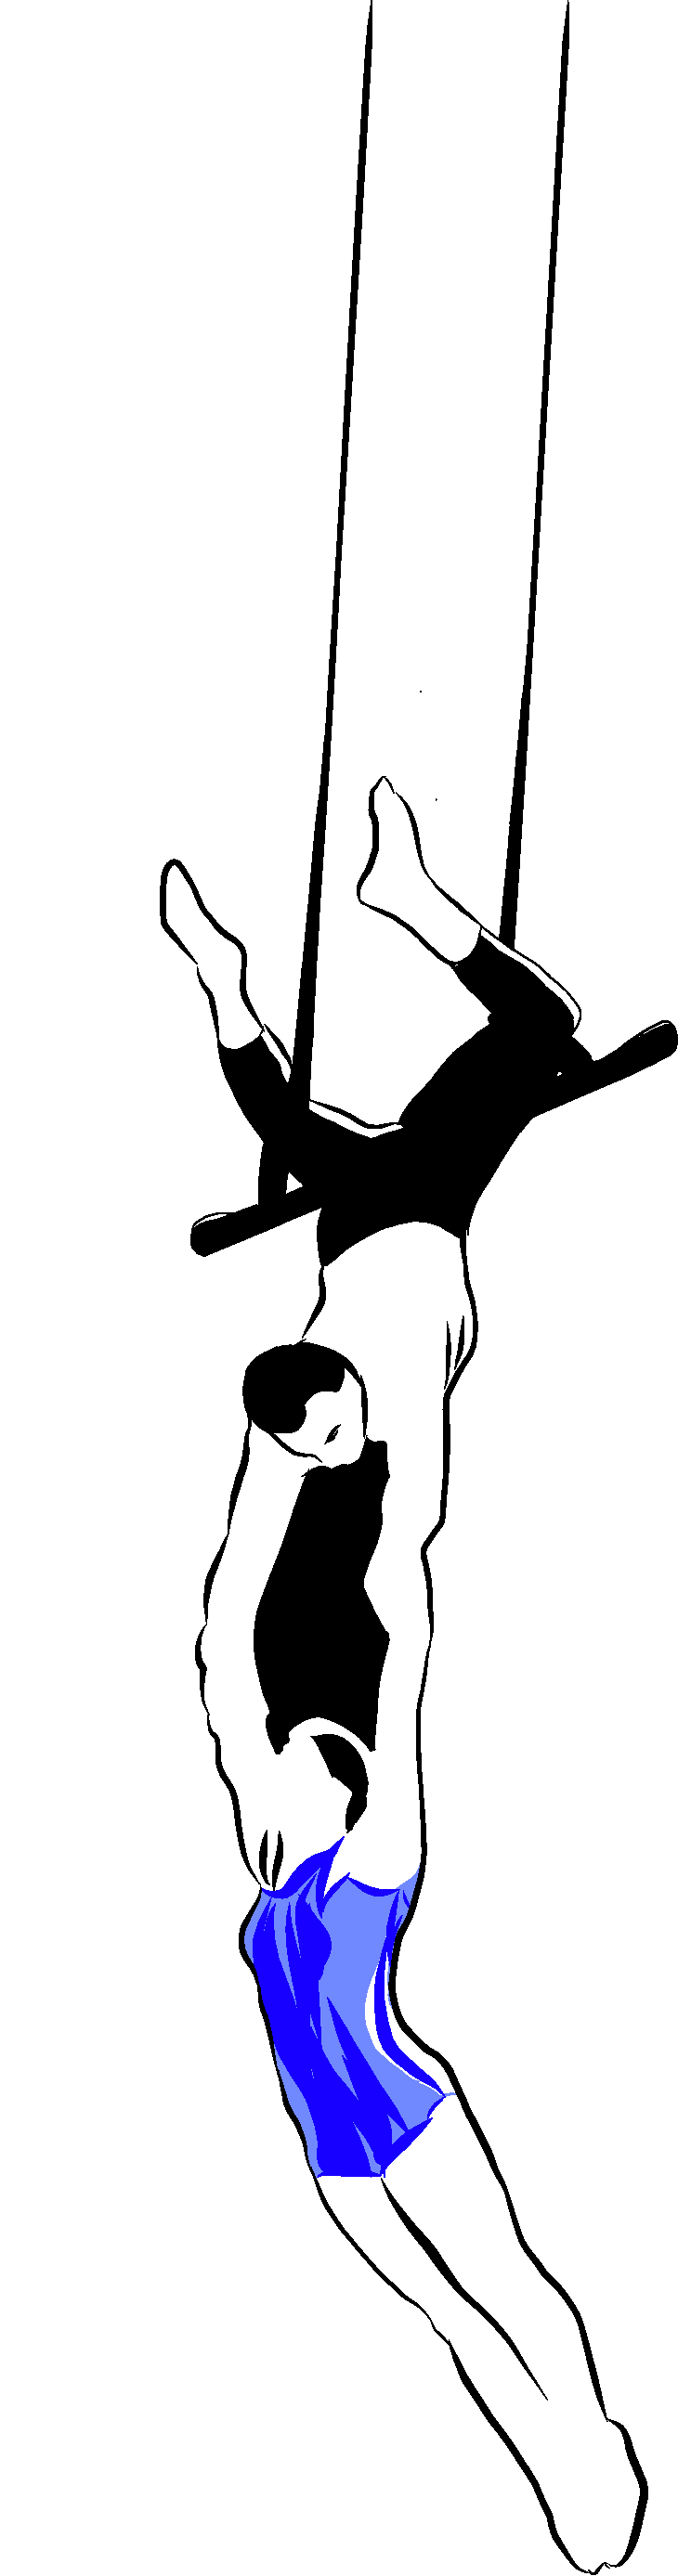
\includegraphics[width=2in]{images/duo_trapeze.pdf}
\newpage
\bversenonum \firstletter{I}{n the style of} \textit{Where the Wild Things Are}, write or illustrate instructions for how to live in a world where universal basic income is the norm because so many jobs have been automated.
\newpages{1}
\bversenonum \firstletter{I}{n the style of} Maurice Sendak, or any other children's author you fant'sy, write sex-positive guidelines for children\footnote{Let's be honest. Some adults need this, too.} on when it's appropriate to masturbate.
\newpage
\hfill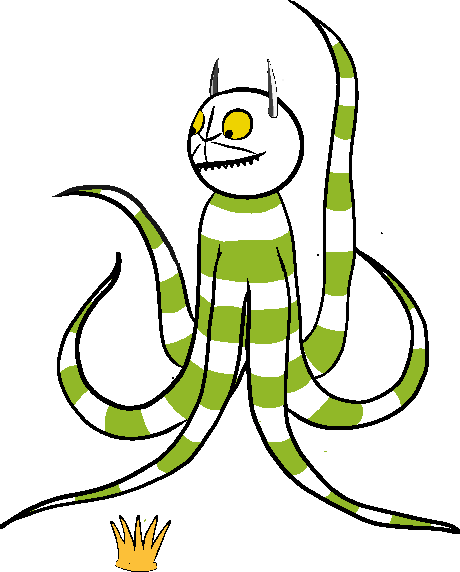
\includegraphics[width=4in]{images/wild_things.pdf}
\newpage
\bversenonum \firstletter{I}{n the style of} your favorite children's book, write or illustrate your favorite set of ethical guidelines (utilitarianism, deontology, \textit{etc.}).
\newpages{1}
\bversenonum \firstletter{I}{n the style of} Dr.~Seuss, write or illustrate guidelines on how to be ethically polyamorous.
\newpages{1}
\bversenonum \firstletter{W}{rite} a parable about unicorns.
\newpages{1}
\bversenonum \firstletter{I}{n limerick form}, write or illustrate the story of the moon landing.
\newpages{1}
\bversenonum \firstletter{W}{hat} are the `Ten Commandments' of Whimsy?
\newpages{1}
\bversenonum \firstletter{I}{n the style of} your favorite poet, or as an illustrated guide, write general instructions for terraforming Mars.
\newpages{1}
\bversenonum \firstletter{I}{n the style of} Dr.~Seuss, write or illustrate the best piece of advice someone has ever offered you.


%\end{@twocolumnfalse}

\end{document}